\begin{figure}
  \centering
  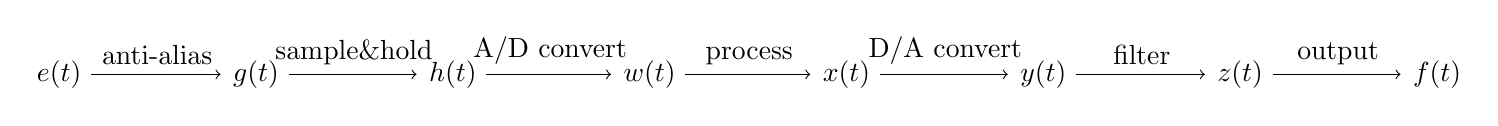
\begin{tikzpicture}[->,shorten >=1pt,auto,node distance=2.5cm]
    \node (e) {$e(t)$};
    \node (g) [right of=e] {$g(t)$};
    \node (h) [right of=g] {$h(t)$};
    \node (w) [right of=h] {$w(t)$};
    \node (x) [right of=w] {$x(t)$};
    \node (y) [right of=x] {$y(t)$};
    \node (z) [right of=y] {$z(t)$};
    \node (f) [right of=z] {$f(t)$};
    \path (e) edge node {anti-alias} (g);
    \path (g) edge node {sample\&hold} (h);
    \path (h) edge node {A/D convert} (w);
    \path (w) edge node {process} (x);
    \path (x) edge node {D/A convert} (y);
    \path (y) edge node {filter} (z);
    \path (z) edge node {output} (f);
  \end{tikzpicture}

  \caption{Signal processing chain}
\end{figure}